\documentclass[10pt]{beamer}

\usepackage{packages}
\title{Exercício Programa 1}
\subtitle{Escalonador de processos}
\institute{IME-USP}
\author{Lucas Paiolla Forastiere e Marcos Siolin Martins}
\date{05 de outubro de 2020}

\begin{document}
    \maketitle
    \section{Shell}
    \begin{frame}{Arquitetura do Shell}
      O shell segue a arquitetura sugerida em aula, tendo sido implementado apenas no arquivo \texttt{bccsh.c}.

      Conta com um loop principal em que lê um comando por iteração e executa esse comando internamente por meio de chamadas de sistema ou realiza a invocação externa do binário informado até que um sinal \texttt{EOF} seja emitido pelo usuário (pressionar as teclas \texttt{CTRL+D}).
    \end{frame}
    \begin{frame}{Arquitetura do Shell}
      Além disso algumas decisões de projetos foram tomadas, entre elas:
      \begin{itemize}
        \justifying
        \item A função \texttt{read\_command(command, parameters)} recebe o comando digitado pelo usuário, usando a função \texttt{readline()}, e devolve o comando na variável \texttt{command} e os parâmetros na variável \texttt{parameters}. Por definição, \texttt{parameters[0] = command};
        \item A função \texttt{readline()} aloca a memória necessária. Guardamos seu retorno no histórico usando \texttt{add\_history()} e tratamos seu retorno substituindo espaços em branco pelo caractere `\textbackslash 0' e mudando os ponteiros de \texttt{parameters} para o começo de cada parâmetro na string.
      \end{itemize}
    \end{frame}
    \begin{frame}{Arquitetura do Shell}
      \begin{itemize}
        \justifying
        \item Todos os arrays que não são alocados por funções externas são alocados estaticamente com valor máximo definido por diretivas \texttt{\#define}:
        \begin{itemize}
          % \vspace{-0.25in}
          \item \texttt{CUR\_DIR\_SIZE}: tamanho máximo do nome do diretório;
          \item \texttt{PROMPT\_SIZE}: tamanho máximo da string exibida no prompt;
          \item \texttt{MAX\_PARAMETERS}: quantidade máxima de parâmetros.
        \end{itemize}
        \item Por fim, implementamos a chamada de sistema \texttt{mkdir} passando como parâmetro a constante \texttt{S\_IRWXU} que dá ao usuário todas as permissões sobre aquele diretório.
      \end{itemize}
    \end{frame}
    \section{Escalonadores}
    \subsection{Implementação}
    \begin{frame}{Implementação dos Escalonadores}
    Inicialmente, todas as threads que eventualmente chegarão no sistema são carregadas do arquivo de entrada, criadas e ficam bloqueadas até que o escalonador lhes dê a permissão de rodar.

    Para fazer esse gerenciamento das threads, existe um array de mutex (chamado \texttt{mutex}) em
        que cada mutex está associado a uma thread. Se o mutex está liberado, então a thread pode
        rodar. Caso contrário, a thread fica bloqueada. Usamos os mutex da biblioteca
        \texttt{pthread} para fazer esse gerenciamento, juntamente com as funções \texttt{pthread\_lock} e \texttt{pthread\_unlock}.
    \end{frame}
    \begin{frame}{Implementação dos Escalonadores}
        A variável inteira chamada \texttt{semaforo} possui valor igual à thread que está em execução no momento (decidimos que apenas uma thread executaria por vez).

        Essa variável é gerenciada pela função \texttt{setSemaforo(value)},
        que recebe o valor da thread que executará e bloqueia a antiga
        thread para liberar a nova (caso o valor passado seja -1,
        então isso indica que nenhuma thread está em execução no momento).
    \end{frame}

    \begin{frame}{Implementação dos Escalonadores}
        Decidimos também criar uma \texttt{struct} para os processos, para
        armazenar algumas informações de cada processo. Como o tempo em que ela terminou
        de executar e as propriedades informadas no arquivo de trace.

        Esses processos ficam em um array chamado \texttt{processos} que possui tamanho
        máximo igual a \texttt{nmax}. Assumimos que o número máximo de processos é
        $1000$, mas deixamos \texttt{nmax} como $1024$ para ter uma folga.

        Todas as variáveis e funções de uso amplo foram colocadas no arquivo
        \texttt{util.h} e cada escalonador foi implementado em um arquivo próprio.        
    \end{frame}

    \begin{frame}{Implementação dos Escalonadores}
        Por fim, o arquivo \texttt{ep1.c} possui a função \texttt{main} e a função
        \texttt{busy}, que é a função executada por cada uma das threads.

        O consumo de CPU realizado por ela advém da função \texttt{sched\_getcpu()},
        que retorna a CPU atual em que a thread está executando. Nos nossos testes,
        esse uso foi de $100\%$ do núcleo para os escalonadores \texttt{FCFS} e \texttt{SRTN}. No \texttt{round robin} a ocorrência massiva de preempções dificulta a visualização de qual CPU está sendo usada.

    \end{frame}
    \begin{frame}{Implementação dos Escalonadores - Tempo}
        Sobre o tempo da simulação, o próprio escalonador controla o tempo passado 
        através do uso da função \texttt{usleep(t)} que coloca o escalonador para ``dormir''
        por (pelo menos) $t$ microssegundos. Quando o escalonador ``acorda'' se passaram pelo
        menos $t$ microssegundos e assumimos que exatamente $t$ microssegundos se passaram (o erro cometido por \texttt{usleep} é pequeno de acordo com a documentação).

        A variável global \texttt{cur\_time} controla quantos segundos na simulação se passaram.
        Ela começa com valor igual ao $t_0$ do primeiro processo (avançamos a simulação para o ponto em que o primeiro processo chega).
    \end{frame}
    \begin{frame}{Implementação dos Escalonadores - FCFS}
        No FCFS, aproveitamos a própria fila de processos carregada na entrada para
        simular a ordem dos processos.

        Usamos uma variável \texttt{atual} para controlar o índice da thread que 
        está executando no momento e vamos atualizando o tempo que ela ficou 
        executando conforma a simulação avança.

        Além disso, também mantemos uma variável \texttt{prox} para dizer qual é
        o próximo processo que vai chegar na simulação. Enquando o tempo atual da
        simulação é igual ao $t_0$ de \texttt{prox} indicamos a chegada dele e
        incrementamos a variável.

    \end{frame}

    \begin{frame}{Implementação dos Escalonadores - SRTN}
        No SRTN, usamos um vetor \texttt{fila} que guarda os índices de cada thread.

        A variável \texttt{prox} tem o mesmo papel que no FCFS, assim como
        \texttt{atual}.

        A variável \texttt{ini} aponta para o começo da fila e, por definição,
        \texttt{fila[ini-1]} é o processo que está executando no momento.

        A variável \texttt{fim} aponta para a última posição não ocupada da fila e,
        por definição, \texttt{fila[fim]} é sempre igual a -1.

        Além disso, esse escalonador conta com a função \texttt{insere\_na\_fila}, que
        insere o processo que acabou de chegar no seu lugar apropriado na fila
        (ordenado pelo tempo restante de execução) e atualiza os valores de
        \texttt{ini} e \texttt{fim}.
    \end{frame}

    \begin{frame}{Implementação dos Escalonadores - Round Robin}
        No Round Robin, a fila de processos carregada na entrada é reaproveitada para simular a ordem dos processos.

        As variáveis \texttt{atual} e \texttt{prox} cumprem o mesmo papel que cumpriam nos outros dois escalonadores,
        enquanto a variável \texttt{tempo\_dormindo} controla quantos microssegundos além do segundo atual já se passaram.

        O \texttt{quantum} é definido em um \texttt{\#define} e é dado em microssegundos. Testamos para \texttt{quantum = 0.05s}.

        A variável \texttt{minimo} assegura que o escalonador não dormirá por \texttt{quantum} se o tempo para o processo terminar é menor que isso.

        A variável \texttt{todos\_terminaram} controla se todos os processos já encerraram sua execução.
    \end{frame}

    \subsection{Experimentos}
    \begin{frame}{Arquivo de Trace: 10 processos - Mudanças de contexto}
        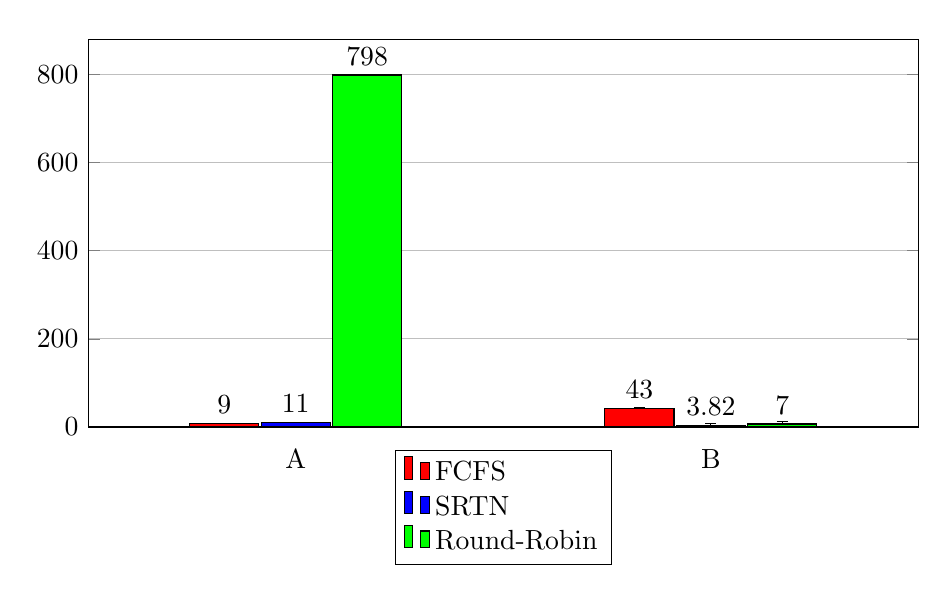
\begin{tikzpicture}
              \begin{axis}[
                  width  = 1.00*\textwidth,
                  height = 6.5cm,
                  major x tick style = transparent,
                  ybar=2*\pgflinewidth,
                  bar width=25pt,
                  ymajorgrids = true,
                  symbolic x coords={A,B},
                  xtick = data,
                  scaled y ticks = false,
                  enlarge x limits=0.50,
                  ymin=0,
                  legend cell align=left,
                  legend style={at={(0.5,-0.06)},anchor=north},
                  nodes near coords, 
                  nodes near coords align={anchor=south},%Move values in bar
                  totals/.style={nodes near coords align={anchor=north}},
                  x tick label style={anchor=south,yshift=-0.5cm},
              ]

              \addplot[style={fill=red},
                error bars/.cd,
                y dir=both,
                y explicit]
              coordinates {
                  (A, 9)
                  (B, 43) += (0,2) -= (0,1)
              };

              \addplot[style={fill=blue},
                error bars/.cd,
                y dir=both,
                y explicit]
              coordinates {
                   (A, 11)
                   (B, 3.82) += (0,5) -= (0,2)
              };

              \addplot[style={fill=green},
                error bars/.cd,
                y dir=both,
                y explicit]
              coordinates {
                   (A,798)
                   (B,7) += (0,5) -= (0,2)
              };


              \legend{FCFS, SRTN, Round-Robin}
            \end{axis}
        \end{tikzpicture}
    \end{frame}

    \begin{frame}{Arquivo de Trace: 100 processos - Mudanças de contexto}
        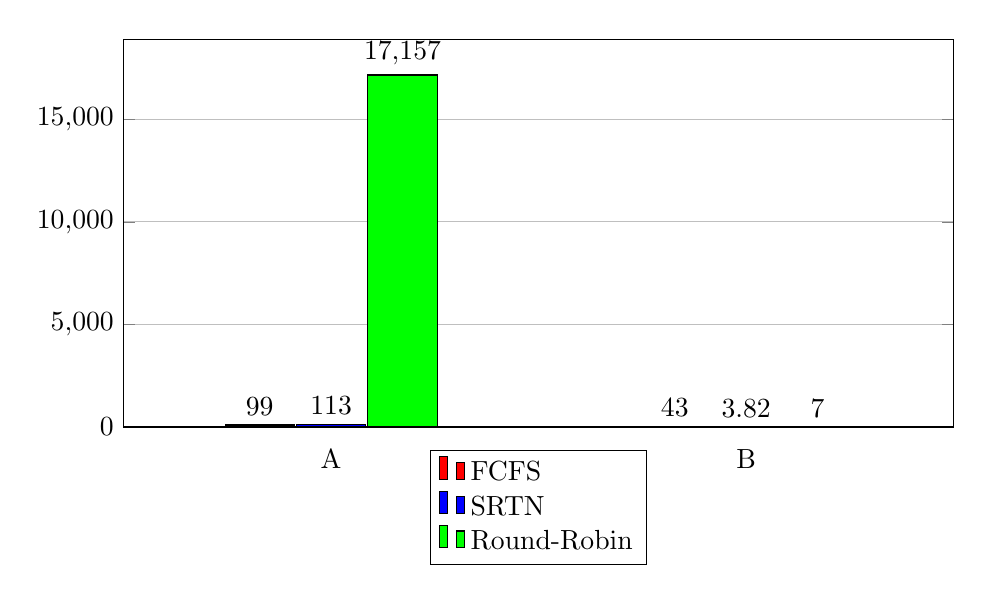
\begin{tikzpicture}
              \begin{axis}[
                  width  = 1.00*\textwidth,
                  height = 6.5cm,
                  major x tick style = transparent,
                  ybar=2*\pgflinewidth,
                  bar width=25pt,
                  ymajorgrids = true,
                  symbolic x coords={A,B},
                  xtick = data,
                  scaled y ticks = false,
                  enlarge x limits=0.50,
                  ymin=0,
                  legend cell align=left,
                  legend style={at={(0.5,-0.06)},anchor=north},
                  nodes near coords, 
                  nodes near coords align={anchor=south},%Move values in bar
                  totals/.style={nodes near coords align={anchor=north}},
                  x tick label style={anchor=south,yshift=-0.5cm},
              ]

              \addplot[style={fill=red},
                error bars/.cd,
                y dir=both,
                y explicit]
              coordinates {
                  (A, 99)
                  (B, 43) += (0,2) -= (0,1)
              };

              \addplot[style={fill=blue},
                error bars/.cd,
                y dir=both,
                y explicit]
              coordinates {
                   (A,113)
                   (B,3.82) += (0,5) -= (0,2)
              };

              \addplot[style={fill=green},
                error bars/.cd,
                y dir=both,
                y explicit]
              coordinates {
                   (A,17157)
                   (B,7) += (0,5) -= (0,2)
              };

              \legend{FCFS, SRTN, Round-Robin}
            \end{axis}
        \end{tikzpicture}
    \end{frame}

    \begin{frame}{Arquivo de Trace: 1000 processos - Mudanças de contexto}
        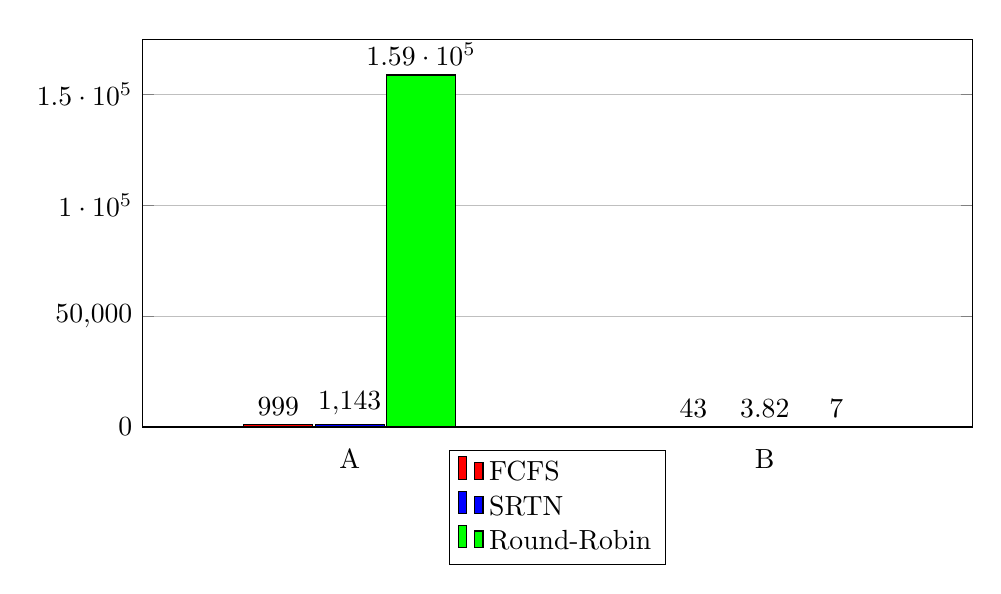
\begin{tikzpicture}
              \begin{axis}[
                  width  = 1.00*\textwidth,
                  height = 6.5cm,
                  major x tick style = transparent,
                  ybar=2*\pgflinewidth,                  
                  bar width=25pt,                  
                  ymajorgrids = true,
                  symbolic x coords={A,B},
                  xtick = data,
                  scaled y ticks = false,
                  enlarge x limits=0.50,
                  ymin=0,
                  legend cell align=left,
                  legend style={at={(0.5,-0.06)},anchor=north},
                  nodes near coords, 
                  nodes near coords align={anchor=south},%Move values in bar
                  totals/.style={nodes near coords align={anchor=north}},
                  x tick label style={anchor=south,yshift=-0.5cm},
              ]

              \addplot[style={fill=red},
                error bars/.cd,
                y dir=both,
                y explicit]
              coordinates {
                  (A, 999)
                  (B, 43) += (0,2) -= (0,1)
              };

              \addplot[style={fill=blue},
                error bars/.cd,
                y dir=both,
                y explicit]
              coordinates {
                   (A,1143)
                   (B,3.82) += (0,5) -= (0,2)
              };

              \addplot[style={fill=green},
                error bars/.cd,
                y dir=both,
                y explicit]
              coordinates {
                   (A,158657)
                   (B,7) += (0,5) -= (0,2)
              };

              \legend{FCFS, SRTN, Round-Robin}
            \end{axis}
        \end{tikzpicture}
    \end{frame}
    \begin{frame}{Arquivo de Trace: 10 processos - Deadlines}
        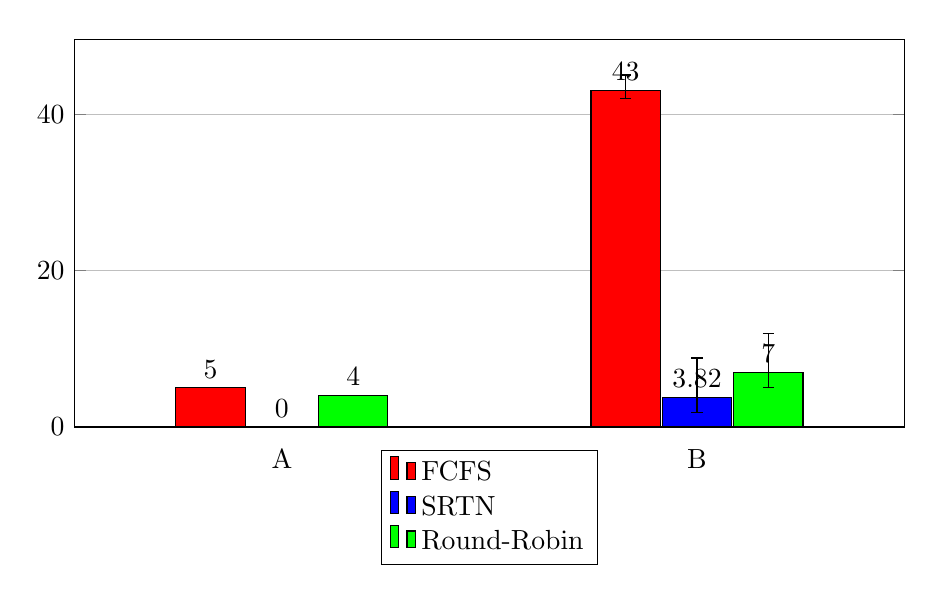
\begin{tikzpicture}
              \begin{axis}[
                  width  = 1.00*\textwidth,
                  height = 6.5cm,
                  major x tick style = transparent,
                  ybar=2*\pgflinewidth,
                  bar width=25pt,
                  ymajorgrids = true,
                  symbolic x coords={A,B},
                  xtick = data,
                  scaled y ticks = false,
                  enlarge x limits=0.50,
                  ymin=0,
                  legend cell align=left,
                  legend style={at={(0.5,-0.06)},anchor=north},
                  nodes near coords, 
                  nodes near coords align={anchor=south},%Move values in bar
                  totals/.style={nodes near coords align={anchor=north}},
                  x tick label style={anchor=south,yshift=-0.5cm},
              ]

              \addplot[style={fill=red},
                error bars/.cd,
                y dir=both,
                y explicit]
              coordinates {
                  (A, 5)
                  (B, 43) += (0,2) -= (0,1)
              };

              \addplot[style={fill=blue},
                error bars/.cd,
                y dir=both,
                y explicit]
              coordinates {
                   (A, 0)
                   (B, 3.82) += (0,5) -= (0,2)
              };

              \addplot[style={fill=green},
                error bars/.cd,
                y dir=both,
                y explicit]
              coordinates {
                   (A,4)
                   (B,7) += (0,5) -= (0,2)
              };


              \legend{FCFS, SRTN, Round-Robin}
            \end{axis}
        \end{tikzpicture}
    \end{frame}

    \begin{frame}{Arquivo de Trace: 100 processos - Deadlines}
        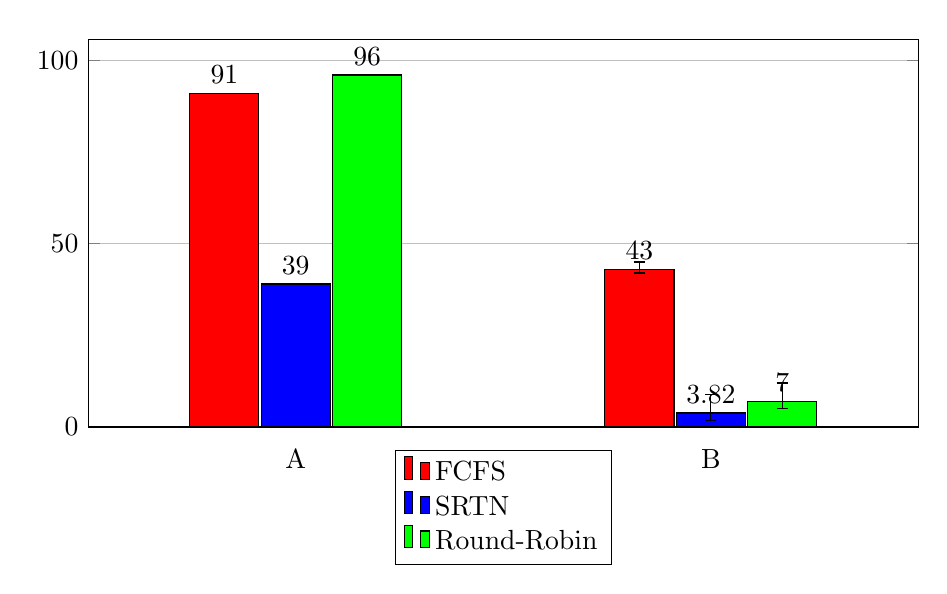
\begin{tikzpicture}
              \begin{axis}[
                  width  = 1.00*\textwidth,
                  height = 6.5cm,
                  major x tick style = transparent,
                  ybar=2*\pgflinewidth,
                  bar width=25pt,
                  ymajorgrids = true,
                  symbolic x coords={A,B},
                  xtick = data,
                  scaled y ticks = false,
                  enlarge x limits=0.50,
                  ymin=0,
                  legend cell align=left,
                  legend style={at={(0.5,-0.06)},anchor=north},
                  nodes near coords, 
                  nodes near coords align={anchor=south},%Move values in bar
                  totals/.style={nodes near coords align={anchor=north}},
                  x tick label style={anchor=south,yshift=-0.5cm},
              ]

              \addplot[style={fill=red},
                error bars/.cd,
                y dir=both,
                y explicit]
              coordinates {
                  (A, 91)
                  (B, 43) += (0,2) -= (0,1)
              };

              \addplot[style={fill=blue},
                error bars/.cd,
                y dir=both,
                y explicit]
              coordinates {
                   (A,39)
                   (B,3.82) += (0,5) -= (0,2)
              };

              \addplot[style={fill=green},
                error bars/.cd,
                y dir=both,
                y explicit]
              coordinates {
                   (A,96)
                   (B,7) += (0,5) -= (0,2)
              };


              \legend{FCFS, SRTN, Round-Robin}
            \end{axis}
        \end{tikzpicture}
    \end{frame}

    \begin{frame}{Arquivo de Trace: 1000 processos - Deadlines}
        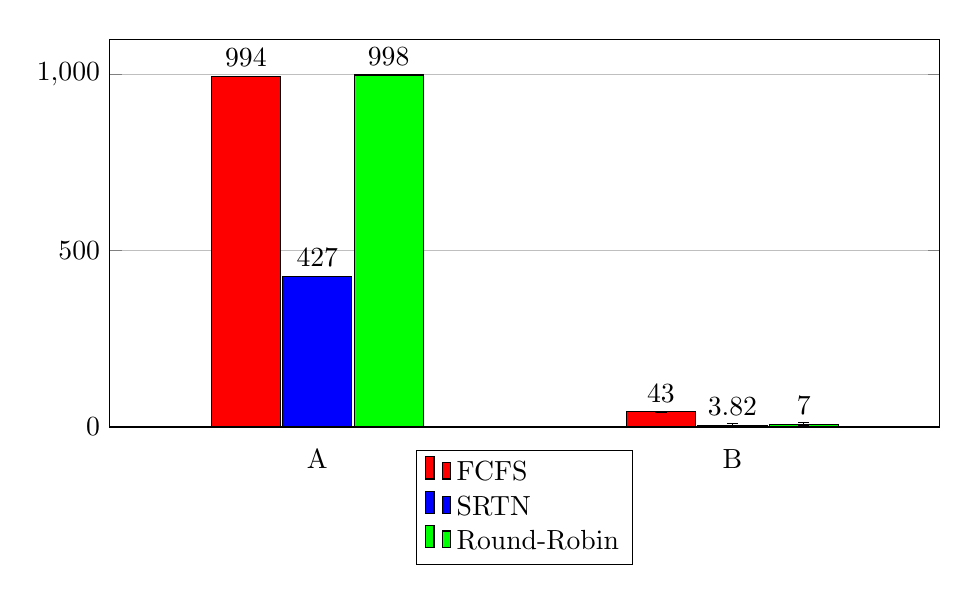
\begin{tikzpicture}
              \begin{axis}[
                  width  = 1.00*\textwidth,
                  height = 6.5cm,
                  major x tick style = transparent,
                  ybar=2*\pgflinewidth,
                  bar width=25pt,
                  ymajorgrids = true,
                  symbolic x coords={A,B},
                  xtick = data,
                  scaled y ticks = false,
                  enlarge x limits=0.50,
                  ymin=0,
                  legend cell align=left,
                  legend style={at={(0.5,-0.06)},anchor=north},
                  nodes near coords, 
                  nodes near coords align={anchor=south},%Move values in bar
                  totals/.style={nodes near coords align={anchor=north}},
                  x tick label style={anchor=south,yshift=-0.5cm},
              ]

              \addplot[style={fill=red},
                error bars/.cd,
                y dir=both,
                y explicit]
              coordinates {
                  (A, 994)
                  (B, 43) += (0,2) -= (0,1)
              };

              \addplot[style={fill=blue},
                error bars/.cd,
                y dir=both,
                y explicit]
              coordinates {
                   (A,427)
                   (B,3.82) += (0,5) -= (0,2)
              };

              \addplot[style={fill=green},
                error bars/.cd,
                y dir=both,
                y explicit]
              coordinates {
                   (A,998)
                   (B,7) += (0,5) -= (0,2)
              };


              \legend{FCFS, SRTN, Round-Robin}
            \end{axis}
        \end{tikzpicture}
    \end{frame}
    \begin{frame}{Conclusões dos experimentos}
        \begin{enumerate}
        \end{enumerate}
    \end{frame}

\end{document}
